\documentclass{beamer}
\newif\ifbeamer\beamertrue
\usepackage{amssymb,amsmath,stmaryrd,txfonts,mathrsfs,amsthm}
\usepackage[all,2cell]{xy}
\usepackage[neveradjust]{paralist}
\usepackage{hyperref}
\usepackage{mathtools}
\usepackage{tikz}
\usetikzlibrary{trees}
\usetikzlibrary{topaths}
\usetikzlibrary{decorations}
\usetikzlibrary{decorations.pathreplacing}
\usetikzlibrary{decorations.pathmorphing}
\usetikzlibrary{decorations.markings}
\usetikzlibrary{matrix,backgrounds,folding}
\usetikzlibrary{chains,scopes,positioning,fit}
\usetikzlibrary{arrows,shadows}
\usetikzlibrary{calc} 
\usetikzlibrary{chains}
\usetikzlibrary{shapes,shapes.geometric,shapes.misc}
\usepackage{smbicat}


\makeatletter
\let\ea\expandafter

%% Defining commands that are always in math mode.
\def\mdef#1#2{\ea\ea\ea\gdef\ea\ea\noexpand#1\ea{\ea\ensuremath\ea{#2}}}
\def\alwaysmath#1{\ea\ea\ea\global\ea\ea\ea\let\ea\ea\csname your@#1\endcsname\csname #1\endcsname
  \ea\def\csname #1\endcsname{\ensuremath{\csname your@#1\endcsname}}}

% Script letters
\newcommand{\sA}{\ensuremath{\mathscr{A}}}
\newcommand{\sB}{\ensuremath{\mathscr{B}}}
\newcommand{\sC}{\ensuremath{\mathscr{C}}}
\newcommand{\sD}{\ensuremath{\mathscr{D}}}
\newcommand{\sE}{\ensuremath{\mathscr{E}}}
\newcommand{\sF}{\ensuremath{\mathscr{F}}}
\newcommand{\sG}{\ensuremath{\mathscr{G}}}
\newcommand{\sH}{\ensuremath{\mathscr{H}}}
\newcommand{\sI}{\ensuremath{\mathscr{I}}}
\newcommand{\sJ}{\ensuremath{\mathscr{J}}}
\newcommand{\sK}{\ensuremath{\mathscr{K}}}
\newcommand{\sL}{\ensuremath{\mathscr{L}}}
\newcommand{\sM}{\ensuremath{\mathscr{M}}}
\newcommand{\sN}{\ensuremath{\mathscr{N}}}
\newcommand{\sO}{\ensuremath{\mathscr{O}}}
\newcommand{\sP}{\ensuremath{\mathscr{P}}}
\newcommand{\sQ}{\ensuremath{\mathscr{Q}}}
\newcommand{\sR}{\ensuremath{\mathscr{R}}}
\newcommand{\sS}{\ensuremath{\mathscr{S}}}
\newcommand{\sT}{\ensuremath{\mathscr{T}}}
\newcommand{\sU}{\ensuremath{\mathscr{U}}}
\newcommand{\sV}{\ensuremath{\mathscr{V}}}
\newcommand{\sW}{\ensuremath{\mathscr{W}}}
\newcommand{\sX}{\ensuremath{\mathscr{X}}}
\newcommand{\sY}{\ensuremath{\mathscr{Y}}}
\newcommand{\sZ}{\ensuremath{\mathscr{Z}}}

% Calligraphic letters
\newcommand{\cA}{\ensuremath{\mathcal{A}}}
\newcommand{\cB}{\ensuremath{\mathcal{B}}}
\newcommand{\cC}{\ensuremath{\mathcal{C}}}
\newcommand{\cD}{\ensuremath{\mathcal{D}}}
\newcommand{\cE}{\ensuremath{\mathcal{E}}}
\newcommand{\cF}{\ensuremath{\mathcal{F}}}
\newcommand{\cG}{\ensuremath{\mathcal{G}}}
\newcommand{\cH}{\ensuremath{\mathcal{H}}}
\newcommand{\cI}{\ensuremath{\mathcal{I}}}
\newcommand{\cJ}{\ensuremath{\mathcal{J}}}
\newcommand{\cK}{\ensuremath{\mathcal{K}}}
\newcommand{\cL}{\ensuremath{\mathcal{L}}}
\newcommand{\cM}{\ensuremath{\mathcal{M}}}
\newcommand{\cN}{\ensuremath{\mathcal{N}}}
\newcommand{\cO}{\ensuremath{\mathcal{O}}}
\newcommand{\cP}{\ensuremath{\mathcal{P}}}
\newcommand{\cQ}{\ensuremath{\mathcal{Q}}}
\newcommand{\cR}{\ensuremath{\mathcal{R}}}
\newcommand{\cS}{\ensuremath{\mathcal{S}}}
\newcommand{\cT}{\ensuremath{\mathcal{T}}}
\newcommand{\cU}{\ensuremath{\mathcal{U}}}
\newcommand{\cV}{\ensuremath{\mathcal{V}}}
\newcommand{\cW}{\ensuremath{\mathcal{W}}}
\newcommand{\cX}{\ensuremath{\mathcal{X}}}
\newcommand{\cY}{\ensuremath{\mathcal{Y}}}
\newcommand{\cZ}{\ensuremath{\mathcal{Z}}}

% blackboard bold letters
\newcommand{\lA}{\ensuremath{\mathbb{A}}}
\newcommand{\lB}{\ensuremath{\mathbb{B}}}
\newcommand{\lC}{\ensuremath{\mathbb{C}}}
\newcommand{\lD}{\ensuremath{\mathbb{D}}}
\newcommand{\lE}{\ensuremath{\mathbb{E}}}
\newcommand{\lF}{\ensuremath{\mathbb{F}}}
\newcommand{\lG}{\ensuremath{\mathbb{G}}}
\newcommand{\lH}{\ensuremath{\mathbb{H}}}
\newcommand{\lI}{\ensuremath{\mathbb{I}}}
\newcommand{\lJ}{\ensuremath{\mathbb{J}}}
\newcommand{\lK}{\ensuremath{\mathbb{K}}}
\newcommand{\lL}{\ensuremath{\mathbb{L}}}
\newcommand{\lM}{\ensuremath{\mathbb{M}}}
\newcommand{\lN}{\ensuremath{\mathbb{N}}}
\newcommand{\lO}{\ensuremath{\mathbb{O}}}
\newcommand{\lP}{\ensuremath{\mathbb{P}}}
\newcommand{\lQ}{\ensuremath{\mathbb{Q}}}
\newcommand{\lR}{\ensuremath{\mathbb{R}}}
\newcommand{\lS}{\ensuremath{\mathbb{S}}}
\newcommand{\lT}{\ensuremath{\mathbb{T}}}
\newcommand{\lU}{\ensuremath{\mathbb{U}}}
\newcommand{\lV}{\ensuremath{\mathbb{V}}}
\newcommand{\lW}{\ensuremath{\mathbb{W}}}
\newcommand{\lX}{\ensuremath{\mathbb{X}}}
\newcommand{\lY}{\ensuremath{\mathbb{Y}}}
\newcommand{\lZ}{\ensuremath{\mathbb{Z}}}

% bold letters
\newcommand{\bA}{\ensuremath{\mathbf{A}}}
\newcommand{\bB}{\ensuremath{\mathbf{B}}}
\newcommand{\bC}{\ensuremath{\mathbf{C}}}
\newcommand{\bD}{\ensuremath{\mathbf{D}}}
\newcommand{\bE}{\ensuremath{\mathbf{E}}}
\newcommand{\bF}{\ensuremath{\mathbf{F}}}
\newcommand{\bG}{\ensuremath{\mathbf{G}}}
\newcommand{\bH}{\ensuremath{\mathbf{H}}}
\newcommand{\bI}{\ensuremath{\mathbf{I}}}
\newcommand{\bJ}{\ensuremath{\mathbf{J}}}
\newcommand{\bK}{\ensuremath{\mathbf{K}}}
\newcommand{\bL}{\ensuremath{\mathbf{L}}}
\newcommand{\bM}{\ensuremath{\mathbf{M}}}
\newcommand{\bN}{\ensuremath{\mathbf{N}}}
\newcommand{\bO}{\ensuremath{\mathbf{O}}}
\newcommand{\bP}{\ensuremath{\mathbf{P}}}
\newcommand{\bQ}{\ensuremath{\mathbf{Q}}}
\newcommand{\bR}{\ensuremath{\mathbf{R}}}
\newcommand{\bS}{\ensuremath{\mathbf{S}}}
\newcommand{\bT}{\ensuremath{\mathbf{T}}}
\newcommand{\bU}{\ensuremath{\mathbf{U}}}
\newcommand{\bV}{\ensuremath{\mathbf{V}}}
\newcommand{\bW}{\ensuremath{\mathbf{W}}}
\newcommand{\bX}{\ensuremath{\mathbf{X}}}
\newcommand{\bY}{\ensuremath{\mathbf{Y}}}
\newcommand{\bZ}{\ensuremath{\mathbf{Z}}}

% fraktur letters
\newcommand{\fa}{\ensuremath{\mathfrak{a}}}
\newcommand{\fb}{\ensuremath{\mathfrak{b}}}
\newcommand{\fc}{\ensuremath{\mathfrak{c}}}
\newcommand{\fd}{\ensuremath{\mathfrak{d}}}
\newcommand{\fe}{\ensuremath{\mathfrak{e}}}
\newcommand{\ff}{\ensuremath{\mathfrak{f}}}
\newcommand{\fg}{\ensuremath{\mathfrak{g}}}
\newcommand{\fh}{\ensuremath{\mathfrak{h}}}
\newcommand{\fj}{\ensuremath{\mathfrak{j}}}
\newcommand{\fk}{\ensuremath{\mathfrak{k}}}
\newcommand{\fl}{\ensuremath{\mathfrak{l}}}
\newcommand{\fm}{\ensuremath{\mathfrak{m}}}
\newcommand{\fn}{\ensuremath{\mathfrak{n}}}
\newcommand{\fo}{\ensuremath{\mathfrak{o}}}
\newcommand{\fp}{\ensuremath{\mathfrak{p}}}
\newcommand{\fq}{\ensuremath{\mathfrak{q}}}
\newcommand{\fr}{\ensuremath{\mathfrak{r}}}
\newcommand{\fs}{\ensuremath{\mathfrak{s}}}
\newcommand{\ft}{\ensuremath{\mathfrak{t}}}
\newcommand{\fu}{\ensuremath{\mathfrak{u}}}
\newcommand{\fv}{\ensuremath{\mathfrak{v}}}
\newcommand{\fw}{\ensuremath{\mathfrak{w}}}
\newcommand{\fx}{\ensuremath{\mathfrak{x}}}
\newcommand{\fy}{\ensuremath{\mathfrak{y}}}
\newcommand{\fz}{\ensuremath{\mathfrak{z}}}

% fraktur letters
\newcommand{\fA}{\ensuremath{\mathfrak{A}}}
\newcommand{\fB}{\ensuremath{\mathfrak{B}}}
\newcommand{\fC}{\ensuremath{\mathfrak{C}}}

\mdef\fahat{\hat{\fa}}

% Underline letters
\newcommand{\uA}{\ensuremath{\underline{A}}}
\newcommand{\uB}{\ensuremath{\underline{B}}}
\newcommand{\uC}{\ensuremath{\underline{C}}}
\newcommand{\uD}{\ensuremath{\underline{D}}}
\newcommand{\uE}{\ensuremath{\underline{E}}}
\newcommand{\uF}{\ensuremath{\underline{F}}}
\newcommand{\uG}{\ensuremath{\underline{G}}}
\newcommand{\uH}{\ensuremath{\underline{H}}}
\newcommand{\uI}{\ensuremath{\underline{I}}}
\newcommand{\uJ}{\ensuremath{\underline{J}}}
\newcommand{\uK}{\ensuremath{\underline{K}}}
\newcommand{\uL}{\ensuremath{\underline{L}}}
\newcommand{\uM}{\ensuremath{\underline{M}}}
\newcommand{\uN}{\ensuremath{\underline{N}}}
\newcommand{\uO}{\ensuremath{\underline{O}}}
\newcommand{\uP}{\ensuremath{\underline{P}}}
\newcommand{\uQ}{\ensuremath{\underline{Q}}}
\newcommand{\uR}{\ensuremath{\underline{R}}}
\newcommand{\uS}{\ensuremath{\underline{S}}}
\newcommand{\uT}{\ensuremath{\underline{T}}}
\newcommand{\uU}{\ensuremath{\underline{U}}}
\newcommand{\uV}{\ensuremath{\underline{V}}}
\newcommand{\uW}{\ensuremath{\underline{W}}}
\newcommand{\uX}{\ensuremath{\underline{X}}}
\newcommand{\uY}{\ensuremath{\underline{Y}}}
\newcommand{\uZ}{\ensuremath{\underline{Z}}}

% bars
\newcommand{\Abar}{\ensuremath{\overline{A}}}
\newcommand{\Bbar}{\ensuremath{\overline{B}}}
\newcommand{\Cbar}{\ensuremath{\overline{C}}}
\newcommand{\Dbar}{\ensuremath{\overline{D}}}
\newcommand{\Ebar}{\ensuremath{\overline{E}}}
\newcommand{\Fbar}{\ensuremath{\overline{F}}}
\newcommand{\Gbar}{\ensuremath{\overline{G}}}
\newcommand{\Hbar}{\ensuremath{\overline{H}}}
\newcommand{\Ibar}{\ensuremath{\overline{I}}}
\newcommand{\Jbar}{\ensuremath{\overline{J}}}
\newcommand{\Kbar}{\ensuremath{\overline{K}}}
\newcommand{\Lbar}{\ensuremath{\overline{L}}}
\newcommand{\Mbar}{\ensuremath{\overline{M}}}
\newcommand{\Nbar}{\ensuremath{\overline{N}}}
\newcommand{\Obar}{\ensuremath{\overline{O}}}
\newcommand{\Pbar}{\ensuremath{\overline{P}}}
\newcommand{\Qbar}{\ensuremath{\overline{Q}}}
\newcommand{\Rbar}{\ensuremath{\overline{R}}}
\newcommand{\Sbar}{\ensuremath{\overline{S}}}
\newcommand{\Tbar}{\ensuremath{\overline{T}}}
\newcommand{\Ubar}{\ensuremath{\overline{U}}}
\newcommand{\Vbar}{\ensuremath{\overline{V}}}
\newcommand{\Wbar}{\ensuremath{\overline{W}}}
\newcommand{\Xbar}{\ensuremath{\overline{X}}}
\newcommand{\Ybar}{\ensuremath{\overline{Y}}}
\newcommand{\Zbar}{\ensuremath{\overline{Z}}}
\newcommand{\abar}{\ensuremath{\overline{a}}}
\newcommand{\bbar}{\ensuremath{\overline{b}}}
\newcommand{\cbar}{\ensuremath{\overline{c}}}
\newcommand{\dbar}{\ensuremath{\overline{d}}}
\newcommand{\ebar}{\ensuremath{\overline{e}}}
\newcommand{\fbar}{\ensuremath{\overline{f}}}
\newcommand{\gbar}{\ensuremath{\overline{g}}}
%\newcommand{\hbar}{\ensuremath{\overline{h}}} % whoops, \hbar means something else!
\newcommand{\ibar}{\ensuremath{\overline{\imath}}}
\newcommand{\jbar}{\ensuremath{\overline{\jmath}}}
\newcommand{\kbar}{\ensuremath{\overline{k}}}
\newcommand{\lbar}{\ensuremath{\overline{l}}}
\newcommand{\mbar}{\ensuremath{\overline{m}}}
\newcommand{\nbar}{\ensuremath{\overline{n}}}
%\newcommand{\obar}{\ensuremath{\overline{o}}}
\newcommand{\pbar}{\ensuremath{\overline{p}}}
\newcommand{\qbar}{\ensuremath{\overline{q}}}
\newcommand{\rbar}{\ensuremath{\overline{r}}}
\newcommand{\sbar}{\ensuremath{\overline{s}}}
\newcommand{\tbar}{\ensuremath{\overline{t}}}
\newcommand{\ubar}{\ensuremath{\overline{u}}}
\newcommand{\vbar}{\ensuremath{\overline{v}}}
\newcommand{\wbar}{\ensuremath{\overline{w}}}
\newcommand{\xbar}{\ensuremath{\overline{x}}}
\newcommand{\ybar}{\ensuremath{\overline{y}}}
\newcommand{\zbar}{\ensuremath{\overline{z}}}

% tildes
\newcommand{\Atil}{\ensuremath{\widetilde{A}}}
\newcommand{\Btil}{\ensuremath{\widetilde{B}}}
\newcommand{\Ctil}{\ensuremath{\widetilde{C}}}
\newcommand{\Dtil}{\ensuremath{\widetilde{D}}}
\newcommand{\Etil}{\ensuremath{\widetilde{E}}}
\newcommand{\Ftil}{\ensuremath{\widetilde{F}}}
\newcommand{\Gtil}{\ensuremath{\widetilde{G}}}
\newcommand{\Htil}{\ensuremath{\widetilde{H}}}
\newcommand{\Itil}{\ensuremath{\widetilde{I}}}
\newcommand{\Jtil}{\ensuremath{\widetilde{J}}}
\newcommand{\Ktil}{\ensuremath{\widetilde{K}}}
\newcommand{\Ltil}{\ensuremath{\widetilde{L}}}
\newcommand{\Mtil}{\ensuremath{\widetilde{M}}}
\newcommand{\Ntil}{\ensuremath{\widetilde{N}}}
\newcommand{\Otil}{\ensuremath{\widetilde{O}}}
\newcommand{\Ptil}{\ensuremath{\widetilde{P}}}
\newcommand{\Qtil}{\ensuremath{\widetilde{Q}}}
\newcommand{\Rtil}{\ensuremath{\widetilde{R}}}
\newcommand{\Stil}{\ensuremath{\widetilde{S}}}
\newcommand{\Ttil}{\ensuremath{\widetilde{T}}}
\newcommand{\Util}{\ensuremath{\widetilde{U}}}
\newcommand{\Vtil}{\ensuremath{\widetilde{V}}}
\newcommand{\Wtil}{\ensuremath{\widetilde{W}}}
\newcommand{\Xtil}{\ensuremath{\widetilde{X}}}
\newcommand{\Ytil}{\ensuremath{\widetilde{Y}}}
\newcommand{\Ztil}{\ensuremath{\widetilde{Z}}}
\newcommand{\atil}{\ensuremath{\widetilde{a}}}
\newcommand{\btil}{\ensuremath{\widetilde{b}}}
\newcommand{\ctil}{\ensuremath{\widetilde{c}}}
\newcommand{\dtil}{\ensuremath{\widetilde{d}}}
\newcommand{\etil}{\ensuremath{\widetilde{e}}}
\newcommand{\ftil}{\ensuremath{\widetilde{f}}}
\newcommand{\gtil}{\ensuremath{\widetilde{g}}}
\newcommand{\htil}{\ensuremath{\widetilde{h}}}
\newcommand{\itil}{\ensuremath{\widetilde{\imath}}}
\newcommand{\jtil}{\ensuremath{\widetilde{\jmath}}}
\newcommand{\ktil}{\ensuremath{\widetilde{k}}}
\newcommand{\ltil}{\ensuremath{\widetilde{l}}}
\newcommand{\mtil}{\ensuremath{\widetilde{m}}}
\newcommand{\ntil}{\ensuremath{\widetilde{n}}}
\newcommand{\otil}{\ensuremath{\widetilde{o}}}
\newcommand{\ptil}{\ensuremath{\widetilde{p}}}
\newcommand{\qtil}{\ensuremath{\widetilde{q}}}
\newcommand{\rtil}{\ensuremath{\widetilde{r}}}
\newcommand{\stil}{\ensuremath{\widetilde{s}}}
\newcommand{\ttil}{\ensuremath{\widetilde{t}}}
\newcommand{\util}{\ensuremath{\widetilde{u}}}
\newcommand{\vtil}{\ensuremath{\widetilde{v}}}
\newcommand{\wtil}{\ensuremath{\widetilde{w}}}
\newcommand{\xtil}{\ensuremath{\widetilde{x}}}
\newcommand{\ytil}{\ensuremath{\widetilde{y}}}
\newcommand{\ztil}{\ensuremath{\widetilde{z}}}

% Hats
\newcommand{\Ahat}{\ensuremath{\widehat{A}}}
\newcommand{\Bhat}{\ensuremath{\widehat{B}}}
\newcommand{\Chat}{\ensuremath{\widehat{C}}}
\newcommand{\Dhat}{\ensuremath{\widehat{D}}}
\newcommand{\Ehat}{\ensuremath{\widehat{E}}}
\newcommand{\Fhat}{\ensuremath{\widehat{F}}}
\newcommand{\Ghat}{\ensuremath{\widehat{G}}}
\newcommand{\Hhat}{\ensuremath{\widehat{H}}}
\newcommand{\Ihat}{\ensuremath{\widehat{I}}}
\newcommand{\Jhat}{\ensuremath{\widehat{J}}}
\newcommand{\Khat}{\ensuremath{\widehat{K}}}
\newcommand{\Lhat}{\ensuremath{\widehat{L}}}
\newcommand{\Mhat}{\ensuremath{\widehat{M}}}
\newcommand{\Nhat}{\ensuremath{\widehat{N}}}
\newcommand{\Ohat}{\ensuremath{\widehat{O}}}
\newcommand{\Phat}{\ensuremath{\widehat{P}}}
\newcommand{\Qhat}{\ensuremath{\widehat{Q}}}
\newcommand{\Rhat}{\ensuremath{\widehat{R}}}
\newcommand{\Shat}{\ensuremath{\widehat{S}}}
\newcommand{\That}{\ensuremath{\widehat{T}}}
\newcommand{\Uhat}{\ensuremath{\widehat{U}}}
\newcommand{\Vhat}{\ensuremath{\widehat{V}}}
\newcommand{\What}{\ensuremath{\widehat{W}}}
\newcommand{\Xhat}{\ensuremath{\widehat{X}}}
\newcommand{\Yhat}{\ensuremath{\widehat{Y}}}
\newcommand{\Zhat}{\ensuremath{\widehat{Z}}}
\newcommand{\ahat}{\ensuremath{\hat{a}}}
\newcommand{\bhat}{\ensuremath{\hat{b}}}
\newcommand{\chat}{\ensuremath{\hat{c}}}
\newcommand{\dhat}{\ensuremath{\hat{d}}}
\newcommand{\ehat}{\ensuremath{\hat{e}}}
\newcommand{\fhat}{\ensuremath{\hat{f}}}
\newcommand{\ghat}{\ensuremath{\hat{g}}}
\newcommand{\hhat}{\ensuremath{\hat{h}}}
\newcommand{\ihat}{\ensuremath{\hat{\imath}}}
\newcommand{\jhat}{\ensuremath{\hat{\jmath}}}
\newcommand{\khat}{\ensuremath{\hat{k}}}
\newcommand{\lhat}{\ensuremath{\hat{l}}}
\newcommand{\mhat}{\ensuremath{\hat{m}}}
\newcommand{\nhat}{\ensuremath{\hat{n}}}
\newcommand{\ohat}{\ensuremath{\hat{o}}}
\newcommand{\phat}{\ensuremath{\hat{p}}}
\newcommand{\qhat}{\ensuremath{\hat{q}}}
\newcommand{\rhat}{\ensuremath{\hat{r}}}
\newcommand{\shat}{\ensuremath{\hat{s}}}
\newcommand{\that}{\ensuremath{\hat{t}}}
\newcommand{\uhat}{\ensuremath{\hat{u}}}
\newcommand{\vhat}{\ensuremath{\hat{v}}}
\newcommand{\what}{\ensuremath{\hat{w}}}
\newcommand{\xhat}{\ensuremath{\hat{x}}}
\newcommand{\yhat}{\ensuremath{\hat{y}}}
\newcommand{\zhat}{\ensuremath{\hat{z}}}

%% FONTS AND DECORATION FOR GREEK LETTERS

%% the package `mathbbol' gives us blackboard bold greek and numbers,
%% but it does it by redefining \mathbb to use a different font, so that
%% all the other \mathbb letters look different too.  Here we import the
%% font with bb greek and numbers, but assign it a different name,
%% \mathbbb, so as not to replace the usual one.
\DeclareSymbolFont{bbold}{U}{bbold}{m}{n}
\DeclareSymbolFontAlphabet{\mathbbb}{bbold}
\newcommand{\bbDelta}{\ensuremath{\mathbbb{\Delta}}}
\newcommand{\bbone}{\ensuremath{\mathbbb{1}}}
\newcommand{\bbtwo}{\ensuremath{\mathbbb{2}}}
\newcommand{\bbthree}{\ensuremath{\mathbbb{3}}}

% greek with bars
\newcommand{\albar}{\ensuremath{\overline{\alpha}}}
\newcommand{\bebar}{\ensuremath{\overline{\beta}}}
\newcommand{\gmbar}{\ensuremath{\overline{\gamma}}}
\newcommand{\debar}{\ensuremath{\overline{\delta}}}
\newcommand{\phibar}{\ensuremath{\overline{\varphi}}}
\newcommand{\psibar}{\ensuremath{\overline{\psi}}}
\newcommand{\xibar}{\ensuremath{\overline{\xi}}}
\newcommand{\ombar}{\ensuremath{\overline{\omega}}}

% greek with hats
\newcommand{\alhat}{\ensuremath{\hat{\alpha}}}
\newcommand{\behat}{\ensuremath{\hat{\beta}}}
\newcommand{\gmhat}{\ensuremath{\hat{\gamma}}}
\newcommand{\dehat}{\ensuremath{\hat{\delta}}}

% greek with checks
\newcommand{\alchk}{\ensuremath{\check{\alpha}}}
\newcommand{\bechk}{\ensuremath{\check{\beta}}}
\newcommand{\gmchk}{\ensuremath{\check{\gamma}}}
\newcommand{\dechk}{\ensuremath{\check{\delta}}}

% greek with tildes
\newcommand{\altil}{\ensuremath{\widetilde{\alpha}}}
\newcommand{\betil}{\ensuremath{\widetilde{\beta}}}
\newcommand{\gmtil}{\ensuremath{\widetilde{\gamma}}}
\newcommand{\phitil}{\ensuremath{\widetilde{\varphi}}}
\newcommand{\psitil}{\ensuremath{\widetilde{\psi}}}
\newcommand{\xitil}{\ensuremath{\widetilde{\xi}}}
\newcommand{\omtil}{\ensuremath{\widetilde{\omega}}}

% MISCELLANEOUS SYMBOLS
\mdef\del{\partial}
\mdef\delbar{\overline{\partial}}
\let\sm\wedge
\newcommand{\dd}[1]{\ensuremath{\frac{\partial}{\partial {#1}}}}
\newcommand{\inv}{^{-1}}
\newcommand{\dual}{^{\vee}}
\mdef\hf{\textstyle\frac{1}{2}}
\mdef\thrd{\textstyle\frac{1}{3}}
\mdef\qtr{\textstyle\frac{1}{4}}
\let\meet\wedge
\let\join\vee
\let\dn\downarrow
\newcommand{\op}{^{\mathit{op}}}
\newcommand{\co}{^{\mathit{co}}}
\newcommand{\coop}{^{\mathit{coop}}}
\let\adj\dashv
\SelectTips{cm}{}
\newdir{ >}{{}*!/-10pt/@{>}}    % extra spacing for tail arrows in XYpic
\newcommand{\pushoutcorner}[1][dr]{\save*!/#1+1.2pc/#1:(1,-1)@^{|-}\restore}
\newcommand{\pullbackcorner}[1][dr]{\save*!/#1-1.2pc/#1:(-1,1)@^{|-}\restore}
\let\iso\cong
\let\eqv\simeq
\let\cng\equiv
\mdef\Id{\mathrm{Id}}
\mdef\id{\mathrm{id}}
\alwaysmath{ell}
\alwaysmath{infty}
\alwaysmath{odot}
\def\frc#1/#2.{\frac{#1}{#2}}   % \frc x^2+1 / x^2-1 .
\mdef\ten{\mathrel{\otimes}}
\mdef\bigten{\bigotimes}
\mdef\sqten{\mathrel{\boxtimes}}
\def\pow(#1,#2){\mathop{\pitchfork}(#1,#2)} % powers and
\def\cpw{\mathop{\odot}}                    % copowers
\newcommand{\mathid}{\mbox{id}}
\newcommand{\cat}[1]{\ensuremath{\mathbf{#1}}}


%% OPERATORS
\DeclareMathOperator\lan{Lan}
\DeclareMathOperator\ran{Ran}
\DeclareMathOperator\colim{colim}
\DeclareMathOperator\coeq{coeq}
\DeclareMathOperator\eq{eq}
\DeclareMathOperator\Tot{Tot}
\DeclareMathOperator\cosk{cosk}
\DeclareMathOperator\sk{sk}
\DeclareMathOperator\im{im}
\DeclareMathOperator\Spec{Spec}
\DeclareMathOperator\Ho{Ho}
\DeclareMathOperator\Aut{Aut}
\DeclareMathOperator\End{End}
\DeclareMathOperator\Hom{Hom}
\DeclareMathOperator\Map{Map}

%% TIKZ ARROWS AND HIGHER CELLS
\makeatletter
\def\slashedarrowfill@#1#2#3#4#5{%
  $\m@th\thickmuskip0mu\medmuskip\thickmuskip\thinmuskip\thickmuskip
   \relax#5#1\mkern-7mu%
   \cleaders\hbox{$#5\mkern-2mu#2\mkern-2mu$}\hfill
   \mathclap{#3}\mathclap{#2}%
   \cleaders\hbox{$#5\mkern-2mu#2\mkern-2mu$}\hfill
   \mkern-7mu#4$%
}

\def\Rightslashedarrowfill@{%
  \slashedarrowfill@\Relbar\Relbar\Mapstochar\Rightarrow}
\newcommand\xslashedRightarrow[2][]{%
  \ext@arrow 0055{\Rightslashedarrowfill@}{#1}{#2}}
\def\hTo{\xslashedRightarrow{}}
\def\hToo{\xslashedRightarrow{\quad}}
\let\xhTo\xslashedRightarrow

\pagestyle{empty}

\newcommand{\Rightthreecell}{\RRightarrow}
\newcommand{\Rtwocell}{\Rightarrow}

\tikzstyle{doubletick}=[-implies, double equal sign distance, postaction={decorate},decoration={markings,mark=at position .5 with {\draw[-] (0,-0.1) -- (0,0.1);}}]

\tikzstyle{darrow}=[-implies, double equal sign distance]

\tikzstyle{doubleeq}=[double equal sign distance]


%% ARROWS
% \to already exists
\newcommand{\too}[1][]{\ensuremath{\overset{#1}{\longrightarrow}}}
\newcommand{\ot}{\ensuremath{\leftarrow}}
\newcommand{\oot}[1][]{\ensuremath{\overset{#1}{\longleftarrow}}}
\let\toot\rightleftarrows
\let\otto\leftrightarrows
\let\Impl\Rightarrow
\let\imp\Rightarrow
\let\toto\rightrightarrows
\let\into\hookrightarrow
\let\xinto\xhookrightarrow
\mdef\we{\overset{\sim}{\longrightarrow}}
\mdef\leftwe{\overset{\sim}{\longleftarrow}}
\let\mono\rightarrowtail
\let\leftmono\leftarrowtail
\let\cof\rightarrowtail
\let\leftcof\leftarrowtail
\let\epi\twoheadrightarrow
\let\leftepi\twoheadleftarrow
\let\fib\twoheadrightarrow
\let\leftfib\twoheadleftarrow
\let\cohto\rightsquigarrow
\let\maps\colon
\newcommand{\spam}{\,:\!}       % \maps for left arrows

\newsavebox{\DDownarrowbox}
\savebox{\DDownarrowbox}{\tikz[scale=1.5]{\draw[-implies,double equal
sign distance] (0,.1) -- (0,-.1); \draw (0,.1) -- (0,-.1);}}
\newcommand{\DDownarrow}{\mathrel{\raisebox{-.2em}{\usebox{\DDownarrowbox}}}}

\newsavebox{\RRightarrowbox}
\savebox{\RRightarrowbox}{\tikz[scale=1.5]{\draw[-implies,double equal
sign distance] (-.1,0) -- (.1,0); \draw (-.1,0) -- (.1,0);}}
\newcommand{\RRightarrow}{\mathrel{\raisebox{.2em}{\usebox{\RRightarrowbox}}}}

%\newsavebox{\Rightslashedarrowbox}
%\savebox{\Rightslashedarrowbox}{\tikz[scale=1.5]{\draw[Rightslashedarrow{}] (-.1,0) -- (1,0);}}
%\newcommand{\Rightslashedarrow}{\mathrel{\raisebox{-.2em}%{\usebox{\Rightslashedarrowbox}}}}


%% EXTENSIBLE ARROWS
\let\xto\xrightarrow
\let\xot\xleftarrow
% See Voss' Mathmode.tex for instructions on how to create new
% extensible arrows.
\def\rightarrowtailfill@{\arrowfill@{\Yright\joinrel\relbar}\relbar\rightarrow}
\newcommand\xrightarrowtail[2][]{\ext@arrow 0055{\rightarrowtailfill@}{#1}{#2}}
\let\xmono\xrightarrowtail
\let\xcof\xrightarrowtail
\def\twoheadrightarrowfill@{\arrowfill@{\relbar\joinrel\relbar}\relbar\twoheadrightarrow}
\newcommand\xtwoheadrightarrow[2][]{\ext@arrow 0055{\twoheadrightarrowfill@}{#1}{#2}}
\let\xepi\xtwoheadrightarrow
\let\xfib\xtwoheadrightarrow
% Let's leave the left-going ones until I need them.

%% EXTENSIBLE SLASHED ARROWS
% Making extensible slashed arrows, by modifying the underlying AMS code.
% Arguments are:
% 1 = arrowhead on the left (\relbar or \Relbar if none)
% 2 = fill character (usually \relbar or \Relbar)
% 3 = slash character (such as \mapstochar or \Mapstochar)
% 4 = arrowhead on the left (\relbar or \Relbar if none)
% 5 = display mode (\displaystyle etc)
\def\slashedarrowfill@#1#2#3#4#5{%
  $\m@th\thickmuskip0mu\medmuskip\thickmuskip\thinmuskip\thickmuskip
   \relax#5#1\mkern-7mu%
   \cleaders\hbox{$#5\mkern-2mu#2\mkern-2mu$}\hfill
   \mathclap{#3}\mathclap{#2}%
   \cleaders\hbox{$#5\mkern-2mu#2\mkern-2mu$}\hfill
   \mkern-7mu#4$%
}
% Here's the idea: \<slashed>arrowfill@ should be a box containing
% some stretchable space that is the "middle of the arrow".  This
% space is created as a "leader" using \cleader<thing>\hfill, which
% fills an \hfill of space with copies of <thing>.  Here instead of
% just one \cleader, we use two, with the slash in between (and an
% extra copy of the filler, to avoid extra space around the slash).
\def\rightslashedarrowfill@{%
  \slashedarrowfill@\relbar\relbar\mapstochar\rightarrow}
\newcommand\xslashedrightarrow[2][]{%
  \ext@arrow 0055{\rightslashedarrowfill@}{#1}{#2}}
\mdef\hto{\xslashedrightarrow{}}
\mdef\htoo{\xslashedrightarrow{\quad}}
\let\xhto\xslashedrightarrow

%% To get a slashed arrow in XYpic, do
% \[\xymatrix{A \ar[r]|-@{|} & B}\]

% ISOMORPHISMS
\def\xiso#1{\mathrel{\mathrlap{\smash{\xto[\smash{\raisebox{1.3mm}{$\scriptstyle\sim$}}]{#1}}}\hphantom{\xto{#1}}}}
\def\toiso{\xto{\smash{\raisebox{-.5mm}{$\scriptstyle\sim$}}}}

% SHADOWS
\def\shvar#1#2{{\ensuremath{%
  \hspace{1mm}\makebox[-1mm]{$#1\langle$}\makebox[0mm]{$#1\langle$}\hspace{1mm}%
  {#2}%
  \makebox[1mm]{$#1\rangle$}\makebox[0mm]{$#1\rangle$}%
}}}
\def\sh{\shvar{}}
\def\scriptsh{\shvar{\scriptstyle}}
\def\bigsh{\shvar{\big}}
\def\Bigsh{\shvar{\Big}}
\def\biggsh{\shvar{\bigg}}
\def\Biggsh{\shvar{\Bigg}}

%HIGHER CELLS



% THEOREM-TYPE ENVIRONMENTS, hacked to
%% (a) number all with the same numbers, and
%% (b) have the right names for autoref
\def\defthm#1#2{%
  \newtheorem{#1}{#2}[section]%
  \expandafter\def\csname #1autorefname\endcsname{#2}%
  \expandafter\let\csname c@#1\endcsname\c@thm}
\newtheorem{thm}{Theorem}[section]
\newcommand{\thmautorefname}{Theorem}
\defthm{cor}{Corollary}
\defthm{prop}{Proposition}
\defthm{lem}{Lemma}
\defthm{sch}{Scholium}
\defthm{assume}{Assumption}
\defthm{claim}{Claim}
\defthm{conj}{Conjecture}
\defthm{hyp}{Hypothesis}
\defthm{fact}{Fact}
\theoremstyle{definition}
\defthm{defn}{Definition}
\defthm{notn}{Notation}
\theoremstyle{remark}
\defthm{rmk}{Remark}
\defthm{eg}{Example}
\defthm{egs}{Examples}
\defthm{ex}{Exercise}
\defthm{ceg}{Counterexample}

% How to get QED symbols inside equations at the end of the statements
% of theorems.  AMS LaTeX knows how to do this inside equations at the
% end of *proofs* with \qedhere, and at the end of the statement of a
% theorem with \qed (meaning no proof will be given), but it can't
% seem to combine the two.  Use this instead.
\def\thmqedhere{\expandafter\csname\csname @currenvir\endcsname @qed\endcsname}

% Number numbered lists as (i), (ii), ...
\renewcommand{\theenumi}{(\roman{enumi})}
\renewcommand{\labelenumi}{\theenumi}

%% Labeling that keeps track of theorem-type names.  Superseded by
%% autoref from hyperref, as above, but we keep this in case we are
%% using a journal style file that is incompatible with hyperref.
% 
% \ifx\SK@label\undefined\let\SK@label\label\fi
% \let\your@thm\@thm
% \def\@thm#1#2#3{\gdef\currthmtype{#3}\your@thm{#1}{#2}{#3}}
% \def\xlabel#1{{\let\your@currentlabel\@currentlabel\def\@currentlabel
% {\currthmtype~\your@currentlabel}
% \SK@label{#1@}}\label{#1}}
% \def\xref#1{\ref{#1@}}

% Also number formulas with the theorem counter
\let\c@equation\c@thm
\numberwithin{equation}{section}

% Only show numbers for equations that are actually referenced (or
% whose tags are specified manually) - uses mathtools.
\mathtoolsset{showonlyrefs,showmanualtags}

%% Fix enumerate spacing with paralist.  This has two parts:
%%   1. enable mixing of "old spacing" lists with those adjusted by paralist
%%   2. allow us to specify a number based on which to adjust the spacing
%% For the first, use \killspacingtrue when you want the spacing
%% adjusted, then \killspacingfalse to turn adjustment off.  For the
%% second, use \maxenum=14 to set the widest number you want the
%% spacing to be calculated with.
\newlength\oldleftmargini       % save old spacing
\newlength\oldleftmarginii
\newlength\oldleftmarginiii
\newlength\oldleftmarginiv
\newlength\oldleftmarginv
\newlength\oldleftmarginvi
\newcount\maxenum
\maxenum=7
\newif\ifkillspacing
\def\@adjust@enum@labelwidth{%
  \advance\@listdepth by 1\relax
  \ifkillspacing                % do the paralist thing
    \csname c@\@enumctr\endcsname\maxenum
    \settowidth{\@tempdima}{%
      \csname label\@enumctr\endcsname\hspace{\labelsep}}%
    \csname leftmargin\romannumeral\@listdepth\endcsname
      \@tempdima
  \else                         % otherwise, reset it
    \csname fixspacing\romannumeral\@listdepth\endcsname
  \fi
  \advance\@listdepth by -1\relax}
% these commands, one for each enum level (I couldn't get a generic
% one to work), test whether oldleftmargin has been set yet, and if
% not, set it from leftmargin; otherwise, they reset leftmargin to
% it.  Just setting oldleftmargin to leftmargin in the preamble
% doesn't seem to work.
\def\fixspacingi{\ifnum\oldleftmargini=0\setlength\oldleftmargini\leftmargini\else\setlength\leftmargini\oldleftmargini\fi}
\def\fixspacingii{\ifnum\oldleftmarginii=0\setlength\oldleftmarginii\leftmarginii\else\setlength\leftmarginii\oldleftmarginii\fi}
\def\fixspacingiii{\ifnum\oldleftmarginiii=0\setlength\oldleftmarginiii\leftmarginiii\else\setlength\leftmarginiii\oldleftmarginiii\fi}
\def\fixspacingiv{\ifnum\oldleftmarginiv=0\setlength\oldleftmarginiv\leftmarginiv\else\setlength\leftmarginiv\oldleftmarginiv\fi}
\def\fixspacingv{\ifnum\oldleftmarginv=0\setlength\oldleftmarginv\leftmarginv\else\setlength\leftmarginv\oldleftmarginv\fi}
\def\fixspacingvi{\ifnum\oldleftmarginvi=0\setlength\oldleftmarginvi\leftmarginvi\else\setlength\leftmarginvi\oldleftmarginvi\fi}

%% Fix paralist references, so that we can refer to (1) instead of
%% just 1.
\def\pl@label#1#2{%
  \edef\pl@the{\noexpand#1{\@enumctr}}%
  \pl@lab\expandafter{\the\pl@lab\csname yourthe\@enumctr\endcsname}%
  \advance\@tempcnta1
  \pl@loop}
\def\@enumlabel@#1[#2]{%
  \@plmylabeltrue
  \@tempcnta0
  \pl@lab{}%
  \let\pl@the\pl@qmark
  \expandafter\pl@loop\@gobble#2\@@@
  \ifnum\@tempcnta=1\else
    \PackageWarning{paralist}{Incorrect label; no or multiple
      counters.\MessageBreak The label is: \@gobble#2}%
  \fi
  \expandafter\edef\csname label\@enumctr\endcsname{\the\pl@lab}%
  \expandafter\edef\csname the\@enumctr\endcsname{\the\pl@lab}%
  \expandafter\let\csname yourthe\@enumctr\endcsname\pl@the
  #1}


% GREEK LETTERS, ETC.
\alwaysmath{alpha}
\alwaysmath{beta}
\alwaysmath{gamma}
\alwaysmath{Gamma}
\alwaysmath{delta}
\alwaysmath{Delta}
\alwaysmath{epsilon}
\mdef\ep{\varepsilon}
\alwaysmath{zeta}
\alwaysmath{eta}
\alwaysmath{theta}
\alwaysmath{Theta}
\alwaysmath{iota}
\alwaysmath{kappa}
\alwaysmath{lambda}
\alwaysmath{Lambda}
\alwaysmath{mu}
\alwaysmath{nu}
\alwaysmath{xi}
\alwaysmath{pi}
\alwaysmath{rho}
\alwaysmath{sigma}
\alwaysmath{Sigma}
\alwaysmath{tau}
\alwaysmath{upsilon}
\alwaysmath{Upsilon}
\alwaysmath{phi}
\alwaysmath{Pi}
\alwaysmath{Phi}
\mdef\ph{\varphi}
\alwaysmath{chi}
\alwaysmath{psi}
\alwaysmath{Psi}
\alwaysmath{omega}
\alwaysmath{Omega}
\let\al\alpha
\let\be\beta
\let\gm\gamma
\let\Gm\Gamma
\let\de\delta
\let\De\Delta
\let\si\sigma
\let\Si\Sigma
\let\om\omega
\let\ka\kappa
\let\la\lambda
\let\La\Lambda
\let\ze\zeta
\let\th\theta
\let\Th\Theta
\let\vth\vartheta

\makeatother

% Tikz styles
\tikzstyle{tickarrow}=[->,postaction={decorate},decoration={markings,mark=at position .5 with {\draw[-] (0,-0.1) -- (0,0.1);}},line width=0.50]

% Local Variables:
% mode: latex
% TeX-master: ""
% End:

\tikzcdset{diagrams={ampersand replacement=\&}}
\autodefs{\cDbl\cMonDbl\cMonBicat\cBicat\cMon\fBicat\fDbl\iMon\fMonDbl\fMonBicat}
\def\ubicat{\underline{\cBicat}}

% \usetheme{Warsaw}
% \setbeamertemplate{headline}{}

\usetheme[height=0cm]{Rochester}
\useinnertheme{circles}
\useoutertheme[compress,subsection=false]{miniframes}
\usecolortheme{rose}
\setbeamertemplate{navigation symbols}{}

\title{Constructing symmetric monoidal bicategories functorially}
\author{Michael Shulman \and Linde Wester Hansen}
\date{AMS Sectional Meeting\\UC Riverside\\Applied Category Theory Special Session\\November 9, 2019}

\AtBeginSection[]
{
  \begin{frame}<beamer>{Outline}
    \tableofcontents[currentsection]
  \end{frame}
}

\begin{document}

\begin{frame}
  \maketitle
\end{frame}

\section{Constructing symmetric monoidal bicategories\dots}

\begin{frame}
  \frametitle{Symmetric monoidal bicategories}
  Symmetric monoidal bicategories are everywhere!
  \begin{enumerate}
  \item Rings and bimodules
  \item Sets and spans
  \item Sets and relations
  \item Categories and profunctors
  \item Manifolds and cobordisms
  \item Topological spaces and parametrized spectra
  \item Sets and (decorated/structured) cospans
  \item Sets and open Markov processes
  \item Vector spaces and linear relations
  \end{enumerate}
\end{frame}

\begin{frame}
  \frametitle{What is a symmetric monoidal bicategory?}
    A \alert{symmetric monoidal bicategory} is a bicategory \cB with
    \begin{enumerate}
    \item A functor $\ten : \cB\times \cB\to \cB$
    \item A pseudonatural equivalence $(A \ten B) \ten C \simeq A \ten (B\ten C)$
    \item An invertible modification
      \[\small
        \begin{tikzcd}
          ((AB)C)D \ar[r] \ar[d] \ar[drr,phantom,"\pi\Downarrow"] \& (A(BC))D \ar[r] \& A((BC)D) \ar[d] \\
          (AB)(CD) \ar[rr] \& \& A(B(CD))
        \end{tikzcd}
      \]
  \item\vspace{-.5cm}
    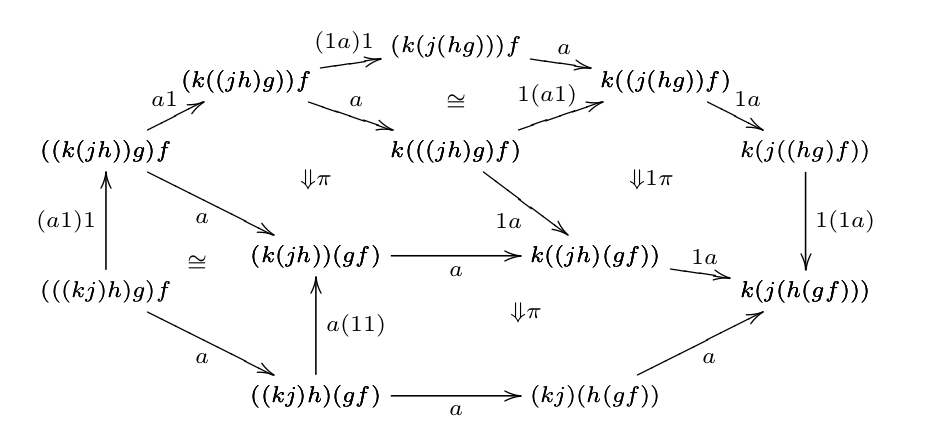
\includegraphics[width=5cm]{associahedron1.png}\;\raisebox{1cm}{$=$}\;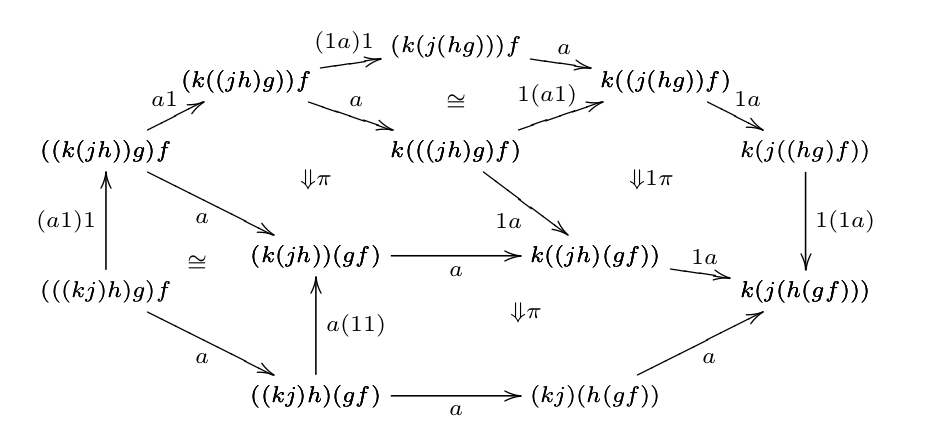
\includegraphics[width=5cm]{associahedron1.png}
  \item more data and axioms for units, braiding, syllepsis\dots
  \end{enumerate}
\end{frame}

\begin{frame}
  \frametitle{Surely it can't be that bad}
  In all the examples I listed before, the monoidal structures
  \begin{enumerate}
  \item tensor product of rings
  \item cartesian product of sets
  \item cartesian product of spaces
  \item disjoint union of sets
  \item \dots
  \end{enumerate}
  are actually associative up to \alert{isomorphism}, with \alert{strictly} commuting pentagons, etc.

  \bigskip
  But a bicategory doesn't know how to talk about isomorphisms, only equivalences!
  We need to add extra data: ring homomorphisms, functions, linear maps, etc.
\end{frame}

\begin{frame}
  \frametitle{Double categories}
  A \alert{double category} is an internal category in Cat.
  It has:
  \begin{enumerate}
  \item objects $A,B,C,\dots$
  \item \alert{loose} morphisms $A\hto B$ that compose weakly
  \item \alert{tight} morphisms $A\to B$ that compose strictly
  \item 2-cells shaped like squares:
    \begin{equation}\label{eq:square}
      \xymatrix{
        A \ar[r]|{|}  \ar[d] \ar@{}[dr]|{\Downarrow}&
        B\ar[d]\\
        C \ar[r]|{|} & D
      }.
    \end{equation}
  \end{enumerate}
  No one can agree on which morphisms to draw horizontally or vertically.
  But ``loose'' and ``tight'' are independent of that choice.
\end{frame}

\begin{frame}
  \frametitle{Symmetric monoidal double categories}
  Double categories, (pseudo) functors, and strictly-natural tight transformations form a 2-category \cDbl.
  \begin{definition}
    A \alert{symmetric monoidal double category} is a symmetric pseudo-monoid in \cDbl.
  \end{definition}
  \begin{itemize}
  \item Coherences are isomorphisms, not equivalences, and diagrams commute strictly.
  \item Hardly more complicated than a pair of ordinary symmetric monoidal categories.
  \end{itemize}
\end{frame}

\begin{frame}
  \frametitle{Symmetric monoidal double categories}
  Symmetric monoidal double categories are everywhere!
  \begin{enumerate}
  \item Rings, bimodules, and ring homomorphisms
  \item Sets, spans, and functions
  \item Sets, relations, and functions
  \item Categories, profunctors, and functors
  \item Manifolds, cobordisms, and diffeomorphisms
  \item Topological spaces, parametrized spectra, and continuous maps
  \item Sets, (decorated/structured) cospans, and functions
  \item Sets, open Markov processes, and functions
  \item Vector spaces, linear relations, and linear transformations
  \end{enumerate}
  \dots but what if what we actually \alert{want} is a monoidal \alert{bicategory}?
\end{frame}


\begin{frame}
  \frametitle{Companions}
  A \alert{companion} of a tight morphism $f:A\to B$ is a loose morphism $\fhat : A\hto B$ and squares
  \begin{equation*}
    \begin{array}{c}
      \xymatrix@-.5pc{
        \ar[r]|-@{|}^-{\smash{\fhat}} \ar[d]_f \ar@{}[dr]|{\Downarrow \epsilon_{\hat{f}} }
        & \ar@{=}[d]\\
        \ar@{=}[r] & }
    \end{array}\quad\text{and}\quad
    \begin{array}{c}
      \xymatrix@-.5pc{
        \ar@{=}[r] \ar@{=}[d] \ar@{}[dr]|{\Downarrow \eta_{\hat{f}}}
        & \ar[d]^f\\
        \ar[r]|-@{|}_-{\smash{\raisebox{-3mm}{$\scriptstyle\fhat$}}} & }
    \end{array}
  \end{equation*}
  such that the following equations hold.
  \begin{align}\label{eq:compeqn}
    \begin{array}{c}
      \xymatrix@-.5pc{
        \ar@{=}[r] \ar@{=}[d] \ar@{}[dr]|{\Downarrow \eta_{\hat{f}}}
        & \ar[d]^f\\
        \ar[r]|-{\fhat} \ar[d]_f \ar@{}[dr]|
        {\Downarrow  \epsilon_{\hat{f}} }
        & \ar@{=}[d]\\
        \ar@{=}[r] & }
    \end{array} &= 
    \begin{array}{c}
      \xymatrix@-.5pc{ \ar@{=}[r] \ar[d]_f
        \ar@{}[dr]|{\Downarrow 1_f} &  \ar[d]^f\\
        \ar@{=}[r] & }
    \end{array}
    &
    \begin{array}{c}
      \xymatrix@-.5pc{
        \ar@{=}[r] \ar@{=}[d] \ar@{}[dr]|{ \Downarrow \eta_{\hat{f}}}&
        \ar[r]|-@{|}^{\fhat}\ar[d]|f \ar@{}[dr]|{\Downarrow  \epsilon_{\hat{f}} }
        & \ar@{=}[d]\\
        \ar[r]|-@{|}_-{\fhat} &
        \ar@{=}[r] &}
%       \xymatrix@-.5pc{
%         \ar[rr]|-@{|}^-{\fhat} \ar@{}[drr]|\iso \ar@{=}[d] &&
%         \ar@{=}[d] \\
%         \ar@{=}[r] \ar@{=}[d] \ar@{}[dr]|\Downarrow &
%         \ar[r]|-@{|}^-{\fhat} \ar[d]_f \ar@{}[dr]|\Downarrow
%         & \ar@{=}[d]\\
%         \ar[r]|-@{|}_-{\fhat} &
%         \ar@{=}[r] &\\
%         \ar[rr]|-@{|}_-{\fhat} \ar@{}[urr]|\iso \ar@{=}[u] &&
%         \ar@{=}[u]}
    \end{array} &=
    \begin{array}{c}
      \xymatrix@-.5pc{
        \ar[r]|-@{|}^-{\fhat} \ar@{=}[d] \ar@{}[dr]|{\Downarrow 1_{\fhat}}
        & \ar@{=}[d]\\
        \ar[r]|-@{|}_-{\fhat} & }
    \end{array}
  \end{align}
  There is also a dual notion of \alert{conjoint}.
  The double categories listed before have companions and conjoints for all tight morphisms\\ (i.e.\ they are \alert{framed bicategories}).
\end{frame}

\begin{frame}
  \frametitle{Constructing symmetric monoidal bicategories}
  \begin{theorem}[S., 2010]
    Let \dD be a symmetric monoidal bicategory whose coherence isomorphisms have loose companions.
    Then the underlying bicategory $\cL\dD$ of objects and loose morphisms is a symmetric monoidal bicategory.
    (And similarly for the monoidal and braided monoidal cases.)
  \end{theorem}
  \begin{proof}
    Lift all the coherences to the companions.
  \end{proof}
  In particular, all the examples listed before are symmetric monoidal bicategories.
\end{frame}

\section{\dots functorially}

\begin{frame}
  \frametitle{What about functors?}
  But we'd also like to be able to construct
  \begin{itemize}
  \item monoidal functors and
  \item monoidal transformations, 
  \item in a way that preserves composition,
  \item and hence preserves things like adjunctions,
  \item \dots
  \end{itemize}
  In other words, what we want is a \alert{functor}
  \[\cL : \cMonDbl \to \cMonBicat .\]
\end{frame}

\begin{frame}
  \frametitle{Functors beget functors}
  Morally, we should have
  \begin{align*}
    \cMonDbl &= \cMon(\cDbl) \\
    \cMonBicat &= \cMon(\cBicat)
  \end{align*}
  and \cMon should be a functor, so that our desired functor
  \[\cL : \cMonDbl \to \cMonBicat \]
  is simply induced by an easier functor
  \[ \cL : \cDbl \to \cBicat. \]
  But \alert{what kind of functors are these?}
\end{frame}

\begin{frame}
  \frametitle{Tricategories?}
  \begin{block}{First answer}
    \cBicat is a \alert{tricategory}, and we can regard \cDbl as a tricategory with no nonidentity 3-cells.
    So \cL should be a tricategory functor.
  \end{block}
  \begin{block}{First problem}
    \begin{itemize}
    \item Constructing a tricategory functor is a lot of work.
    \item More importantly, a monoidal bicategory, as usually defined, is \alert{not} just a ``monoid object in the tricategory \cBicat''.
    \end{itemize}
  \end{block}
  \cBicat is stricter than a general tricategory in several ways, and a definition that makes sense in an arbitrary tricategory would involve a lot of superfluous coherence data when specialized to \cBicat.
\end{frame}

\begin{frame}
  \frametitle{Iconic tricategories?}
  \begin{block}{Second answer}
    \cBicat and \cDbl are \alert{iconic tricategories}: bicategories enriched over the 2-category of bicategories, pseudofunctors, and \alert{icons}.
  \end{block}
  \begin{definition}[Lack 2010]
    An \alert{icon} (\alert{I}dentity \alert{C}omponent \alert{O}plax \alert{N}atural transformation) between pseudofunctors $F,G:\cA\to\cB$ consists of:
    \begin{enumerate}
    \item The assertion that $F(A) = G(A)$ for all objects $A\in\cA$.
    \item For all $\ph:X\to Y$ in \cA, a 2-cell
      \[ \xymatrix{ \mathllap{FX =\;} GX \rtwocell^{F\ph}_{G\ph} & FY \mathrlap{\;= GY} } \]
    \end{enumerate}
  \end{definition}
\end{frame}

\begin{frame}
  \frametitle{Iconic tricategories?}
  % \begin{itemize}
  % \item
    An iconic tricategory is equivalently a tricategory in which composition of 1-cells is strictly associative and unital\\ (though compostion of 2-cells along 0-cells need not be).
  % \item Closely related to the \alert{bicategory-enriched categories} of Verity.
  % \end{itemize}
  \begin{block}{Second problem}
    \cMonBicat is \alert{not} iconic!
  \end{block}
  Composition of monoidal functors of bicategories is not strictly associative.
  For $\cA \xto{F} \cB \xto{G} \cC$, the composite laxator is
  \[ G F X\ten G F Y \xto{G_{\ten}} G(FX\ten FY) \xto{F_{\ten}} GF(X\ten Y) \]
  a composition in \cC, which is a bicategory.
\end{frame}

\begin{frame}[t]
  \frametitle{Third time's the charm}
  \begin{block}{Final answer}
    \fBicat, \fDbl, \fMonBicat, \fMonDbl are all \alert{locally cubical bicategories} (Garner-Gurski 2009): bicategories enriched over the monoidal 2-category \cDbl.
  \end{block}
  \only<1>{\fBicat has:
  \begin{enumerate}
  \item Objects: bicategories
  \item 1-cells: pseudofunctors
  \item loose 2-cells: pseudonatural transformations
  \item tight 2-cells: icons
  \item square 3-cells: cubical modifications
  \end{enumerate}}
\only<2>{\fDbl has:
  \begin{enumerate}
  \item Objects: double categories (with companions)
  \item 1-cells: pseudofunctors
  \item loose 2-cells: strictly-natural tight transformations
  \item tight 2-cells: only identities
  \item square 3-cells: only identities
  \end{enumerate}}
  \only<3>{\fMonBicat has:
  \begin{enumerate}
  \item Objects: monoidal bicategories
  \item 1-cells: monoidal pseudofunctors
  \item loose 2-cells: monoidal pseudonatural transformations
  \item tight 2-cells: monoidal icons
  \item square 3-cells: cubical monoidal modifications
  \end{enumerate}
  In particular, composition of monoidal pseudofunctors is associative up to a \emph{monoidal icon}.}
\end{frame}

\begin{frame}
  \frametitle{Monoids in locally cubical bicategories}
  \begin{theorem}[Hansen--S.]
    Let \fB be a locally cubical bicategory with products, in which composition of 1-cells is strictly associative.
    Then there is a locally cubical bicategory $\iMon(\fB)$ of monoids in \fB.
  \end{theorem}
  Just write down the ordinary definitions of monoidal bicategory, monoidal pseudofunctor, monoidal icon, etc.\ in ``point-free style''.\\
  A 1-strict locally cubical bicategory is (almost) exactly the correct structure in which they make sense.
  \begin{example}\vspace{-.7cm}
  \begin{align*}
    \iMon(\fDbl) &= \fMonDbl\\
    \iMon(\fBicat) &= \fMonBicat
  \end{align*}
\end{example}
\end{frame}

\begin{frame}
  \frametitle{Constructing symmetric monoidal bicategories functorially}
  \begin{theorem}[Hansen-S.]
    Let $F:\fB\to\fC$ be a locally cubical functor that preserves products and also strict 1-cell composition.
    Then there is a locally cubical functor $\iMon(F) : \iMon(\fB) \to \iMon(\fC)$, and similarly for braided and symmetric monoids.
  \end{theorem}
  \begin{example}\vspace{-.7cm}
    \begin{align*}
      \iMon(\fDbl) &\to \iMon(\fBicat)\\
      \mathsf{BrMon}(\fDbl) &\to \mathsf{BrMon}(\fBicat)\\
      \mathsf{SymMon}(\fDbl) &\to \mathsf{SymMon}(\fBicat)
    \end{align*}
  \end{example}
\end{frame}

\begin{frame}
  \frametitle{The fine print, I}
  Monoidal pseudofunctors can be (monoidally) lax, colax, or strong --- and so can monoidal pseudonatural transformations!
    \[
      \xymatrix{
        FX \ten FY \ar[r]^{F_{\ten}} \ar[d]_{\al\ten\al} \drtwocell\omit & F(X\ten Y) \ar[d]^{\al} \\
        GX\ten GY \ar[r]_{G_{\ten}} & G(X\ten Y)
      }
    \]
    \[
      \xymatrix{
        FX \ten FY \ar[r]^{F_{\ten}} \ar[d]_{\al\ten\al} \drtwocell\omit{^} & F(X\ten Y) \ar[d]^{\al} \\
        GX\ten GY \ar[r]_{G_{\ten}} & G(X\ten Y)
      }
    \]
    So we actually have \alert{nine} functors.
\end{frame}

\begin{frame}
  \frametitle{The fine print, II}
  % \begin{itemize}
  % \item We can construct braided and symmetric monoidal bicategories this way, but not properly-sylleptic ones.
% \item
  Bicategories also have a strictly associative \alert{whiskering} operation.
  \[ (\al \ast G)\ast F = \al\ast (G\circ F) \qquad G\ast (F\ast \be) = (G\circ F) \ast \be \]
  But a 1-strict locally cubical bicategory doesn't have such an operation: we have to use $\al \circ 1_F$, which is only \alert{isomorphic} to $\al \ast F$.
  Thus a monoid in $\fBicat$ still has a bit more coherence data than a monoidal bicategory.

  \bigskip
  \structure{Possible fix}: Verity (1992) defined a \alert{multicategory} $\ubicat$ such that $\ubicat$-enriched categories are ``iconic tricategories with strictly associative whiskering''.
  Perhaps there is a similar $\underline{\cDbl}$.
\end{frame}

\begin{frame}
  \frametitle{The fine print, III}
  \begin{itemize}
  \item A monoid in the category of monoids is a commutative monoid.
  \item A monoid in the 2-category of monoidal categories is a\\ braided monoidal category (Joyal--Street 1993).
  \item A monoid in the 2-category of braided monoidal categories is a symmetric monoidal category (Joyal--Street 1993).
  \end{itemize}
  We should similarly have $\iMon(\iMon(\fB)) \simeq \mathsf{BrMon}(\fB)$, etc. ---\\
  but our $\iMon$ can't be iterated, since $\iMon(\fB)$ is no longer 1-strict!

  \bigskip
  The restriction of 1-strictness is surprisingly hard to lift.
  Without it, the coherence diagrams for defining monoids in a locally cubical bicategory end up trying to compose tight and loose 2-cells with each other.
  We need some kind of ``local companions''.
\end{frame}

\end{document}
